\chapter{Background \& Objectives}

\section{Background}
\label{sec:bck_background}
\subsection{Hansard Dataset}
\label{sec:bck_hansard}
The Hansard is a set of documents produced by the British Parliament, which began in the 18th and 19th century. These documents contain reports and details of debates in the House of Commons, going back to the year 1803. Eventually, in 1907, these reports were made official and started being produced by Parliament itself, becoming “The Official Report”, though still unofficially known as Hansard. Along with becoming official, a report was officially defined as being one:
\begin{quote} “which, though not strictly verbatim, is substantially the verbatim report, with repetitions and redundancies omitted and with obvious mistakes corrected, but which on the other hand leaves out nothing that adds to the meaning of the speech or illustrates the argument"\cite{HouseofCommonsInformationOffice2010}
\end{quote}
Hansard is available in a variety of versions. The most commonly used and best known version is the Daily Hansard, which appears each morning and reports the previous day’s proceedings. However, access to this is via an API that only provides the most recent 7 days. For this project, most training and processing will be done on the Historical Hansard dataset, which is a dataset containing all 6 series of Hansard, between 1803 to 2004, though it is expected that some of the older documents will be less useful for this project due to the likelihood of them using outdated speech that would no longer be relevant.

The Historical Hansard Dataset is available online in an XML format. Multiple documents per series are available, each document covering a few days debates at most. It is a large dataset, reaching around 10Gb in size in total. Most of the documents available are scanned from hard copies, rather than typed up directly, meaning there is a possibility of small errors from the scanning process that may have to be dealt with. Additionally, from preliminary investigation, the data itself appears to be only loosely formatted, and each of the six series appear to be formatted in a slightly different way, so any system designed to read this data will have to be capable of dealing with any changes to formatting.

\subsection{Natural Language Processing}
\label{sec:bck_NLP}
Natural Language Processing (NLP) is the exploration of how computers can be used to understand and manipulate natural language text or speech to do useful things\cite{chowdhury2003natural}. Computers are very good at dealing with numbers and performing complex calculations at high speed, but they are not as good at understand spoken or written language. Because of this, a large part of NLP is the act of processing the data, or text, to make it easier for the computer to understand and work with, as well as gathering knowledge on how human beings understand and use language so that appropriate tools and techniques can be developed\cite{chowdhury2003natural}. NLP covers multiple topics, such as \emph{Named Entity Recognition}, \emph{Part of Speech Tagging}, and \emph{Sentence Boundary Disambiguation}. However, the part this project is mainly interested is the act of \emph{Sentiment Analysis}.

Sentiment Analysis, also known as Opinion Mining, is the process of identifying and extracting the opinions expressed in a piece of text\cite{Liu2010}. It aims to determine the attitude of a speaker or writer towards a topic, or the overall polarity of a piece of text. This can be a judgment made by the writer or speaker, in the case of reviews, or the emotional state of the speaker or writer.

A basic version of Sentiment Analysis classifies the polarity of a piece of text, classifying it as either positive, negative or neutral. A more advanced version would be, for example, looking at emotions expressed in the text, classifying it as angry, happy, or sad, as some examples. A basic method used can be to compare a piece to two lists of words, one a list of words that usually denote a positive polarity, and one that usually denotes a negative polarity. A system can then simply count the number of positive and negative words in a piece of text, account for any negation (Saying \emph{not great} would change the word \emph{great} from a positive to a negative word, for instance) and whichever type of word was most common would denote the piece of text’s sentiment. However, this method is likely only useful for those pieces of text where it’s known that strong sentiment is likely to be expressed in a simple enough manner, in text such as a review of a product or film.

Stance Detection is another aspect of Natural Language Processing, similar to Sentiment Analysis. However, the difference here is that Stance Detection sets out to classify the stance of text towards a particular target, or entity. Whereas Sentiment Analysis is the overall mood or polarity of text, Stance Detection specifically looks to see if the text is for, against, or neutral towards something\cite{Augenstein2016}. An example would be detecting the stance of a news article towards the subject it's being written about. This may be more applicable to the Hansard Dataset than Sentiment Analysis as the members of parliament are likely to be expressing some form of stance on a topic that they are debating, but also somewhat more complicated to do, as the subject of the stance must also be discovered from the text, which is not guaranteed to be explicitly stated.

\subsection{Related Work}
\label{sec:bck_related}

In researching the potential design of project, a few relevant pieces of work done by others were discovered, some of which had a useful impact on the design of this project. 

\subsubsection{Towards Sentiment Analysis on Parliamentary Debates in Hansard}
\emph{Towards sentiment analysis on parliamentary debates in Hansard}\cite{Onyimadu2014} is a paper which discussed the progress made by \textbf{Onyimadu \emph{et al}} towards applying classic sentiment analysis techniques to the Hansard dataset, such as word association. The paper details the proposed approach to sentiment analysis, by using \emph{“…heuristic classifiers based on the use of statistical and syntactic clues in the text…”} and using a sentiment lexicon base known as the MPQA corpus (Multi Perspective Question Answering) to identify sentences containing known positive or negative words. They first classify a sentence using this lexicon, annotating sentences as possitve or negative depending on the number of positive or negative words, before then applying syntactic clues to improve the classification, such as the presence of negations, such as \emph{“not”} or \emph{“never”}, and the inclusion of intensifying adverbs such as \emph{“very”}. The paper reports an average of 43\% correctly annotated sentences, claiming that the correctly annotated sentences were those \emph{“…without compound opinions, sarcasm and comparative sentences…”,} showing that the style of debate speech renders their syntactic and lexical based approach insufficient for the task.

This paper demonstrates the need to customize sentiment analysis for the Hansard Dataset, as it shows that the standard techniques used are not applicable to the debate speech. Any design for the project should therefore acknowledge the need to be specifically trained on the Hansard Dataset.

\subsubsection{They Work For You}
\emph{They Work For You}\cite{mySociety} is a website that allowed the user to search for their local MP via post code, and the site can then display the voting patterns for that MP, along with information about how often their votes align with their parties votes, and shows examples of appearances made by that MP and what they said. The source code is publicly available on Github and uses python for a large part of their code base. Whilst it does not appear that they use any form of sentiment analysis, it’s still a good example of the sort of thing that can be done using the parliamentary data, and would likely be well supplemented by my project, allowing them to also show how an MP might speak in debates, as well as how they vote.

This website shows what sort of information tends to be extracted from debates and shows what is usually considered interesting. In addition, it's code is open source and hosted on \href{https://github.com/mysociety/theyworkforyou}{A GitHub Repository}. In addition, it also uses the daily form of Hansard, and so can provide an insight into how to go about parsing data from that source.

\subsubsection{The Fake News Challenge}
\emph{The Fake News Challenge}\cite{FakeNewsChallenge2017} is a challenge set up to explore \emph{"how artificial intelligence technologies could be leveraged to combat fake news."} and aims to eventually produce a tool that can help human fact checkers tell if a news story is a hoax, or intentionally misleading. The first part of the challenge involved the use of Stance Analysis on a series of news articles, comparing the contents of the article with the headline, to tell if the article contents agree with the claims made in the headlines. As the project is set up as a competition, multiple teams submitted solutions to the problem, showing a variety of techniques in solving this problem.

This project is built on the work of \textbf{Ferreira et al.}\cite{Ferreira2016}, who built a dataset based around articles, the claims they are based on, and the stance of the article, where a \emph{For} Stance means the article reports the claim as true, an \emph{Against} Stance means the article reports the claim as false, and an \emph{Observing} stance means the article reports on the claim, but does not report of its veracity.

Stance detection is a potential alternative to Sentiment Analysis for the project. Instead of the basic \emph{Positive} or \emph{Negative} output of Sentiment Analysis, based on just the contents of the text being classified, Stance Analysis compares the contents of two pieces of text to see if they are related to the same topic, and if so, if they agree or disagree. This could be applied to the speech found in Hansard, by comparing the speech of the MP with the topic being debated, to automatically see if they are speaking for or against the topic, or have gone off topic.

\subsection{Technical Research}
\label{sec:bck_tech_research}

Before any form of planning could begin for the project, some research on the kinds of technologies available was required. Three topics had to be researched, namely the language to be used, what methods were available for sentiment analysis, and what was available to extract the data from its original form to something more usable.

For sentiment analysis, and other required NLP tools, the Natural Language Toolkit (NLTK)\cite{Bird2009} was found. This Python package provides methods and classes for a majority of NLP tasks, including everything required for this project. Additionally, it’s well documented, as it is commonly used by other projects that require some form of NLP. This means it would be easy to find solutions to any problem encountered during development, as it is highly likely someone else using the same package has encountered a similar issue and documented a solution online. Due to this, it was quickly decided that the NLTK package would be used for all NLP requirements, which also meant the language to be used would be Python.

There was also a NLP package available for Python called \href{spacy.io}{SpaCy}, which is similar to NLTK. It is, however, newer, and less well documented than NLTK, simply because it is not yet as popular. This means that, should any issues arise, it may be harder to find a solution or any help on the subject. It is possible that in the future SpaCy may prove to be a more useful NLP package, but for the purposes of this project NLTK's commonness wins out.

Once a language was selected, some form of parsing tool had to be discovered. As the data is provided in XML, a commonly used semi-structured database format, the chosen parser solution had to be able to parse XML. An often used package for Python that could do this is “lxml”, a package which could read in XML data structures and translate them into its own set of classes to be used in Python. However, lxml expects well structured data, whereas the hansard dataset is not as well organised. For this reason, it was decided that BeautifulSoup4\cite{Richardson} would be used, a module designed to parse less structured data, in HTML or XML. It makes use of the lxml module, but provides methods that allow the parsing of data whose structure is unknown.

\section{Analysis}
\label{sec:bck_analysis}
Following along from the background research, some decisions were made on how this project would proceed, and what challenges were expected. Additionally, the design of the overall system had to be developed, and the developmental process.

Due to the size and complexity of some of the source data, it was decided that the system would not be able to work directly with the original data without some form of intermediary parsing system. Thus, part of the project was to develop a parser that would get all relevant data from the original files, and reorganize them into a more useful format. It was therefore also necessary to decide on the structure of the data once parsed, and how this data would be stored and accessed by the rest of the system. It would also be necessary to decide what exactly from the original data was relevant to the project.
Additionally, it was important that speech be attributed to the correct member of parliament. It often appeared that the way an MP was referenced in the data would change, going from a full title, honorific and name to just surname. It was important that these different forms of name be recognized as the same person, otherwise speech attributed to just one person would be seen as being said by different people, reducing the accuracy of any searching. This could be done using Named Entity Recognition, an aspect of NLP.

Any form of supervised machine learning method requires training and testing datasets. Due to the nature of the data being used, there are no preexisting sets of annotated data available, and thus the datasets used must be hand annotated. A tool designed to do this must therefore be produced that can assist in this lengthy process, allowing a user to generate a set of annotated data that can then be used to train an Artificial Intelligence.

\subsection{Project Aims}
\label{sec:bck_project_aims}
From the analysis of the problem, a decision needed to be made about what exactly the project will aim to do. This can then be developed further into a proper design later on the developmental process.

The main target of the project is to be able to automatically extract the sentiment expressed in Parliamentary Debates, and track trends in the sentiment expressed by an individual or about a topic. In order to manage this, the project will have to undergo the following tasks:
\begin{itemize}
	\item Download the Hansard Dataset
	\item Extract the relevant information from the dataset
	\item Extract Sentiment from the speech extracted, and save it in a way that can be searched for.
\end{itemize}

These tasks will likely need to be broken down further in order to be efficiently developed, but they represent the overall aims and goals of the project.

\section{Process}
\label{sec:bck_process}
The process selected for this project was Feature Driven Development (FDD), an agile styled methodology designed to focus on delivering working blocks of software repeatedly. Though this methodology is not usually designed for a single developer, it was chosen for its ability to break down the larger tasks of \emph{Develop a fully functioning system} into smaller, easier to digest tasks of \emph{Develop the part of the parser that searches for speech} or \emph{Develop a method of comparing two names}. It began with an overall design of the system, and then this design was broken down into a list of "features", by breaking down the overall design into functional sections, represented by the blocks in the diagram. Each of those is decomposed further into a list of features for each one, which can then be targeted as milestones during development. Because these features are relatively  small, completing them is a small task, and keeping track of the progress on each feature can give a decent report on the progress of the project as a whole.

For version control, git, and Github.com was used to maintain versions of code. This can then also be used as a backup service, with the online version of the code hosted on Github being a form of backup, and allowing the code to be transferred between multiple machines with relative ease.

 A “to-do” page was also maintained on \href{https://trello.com}{Trello}, which is an online resource for producing Kanban style to-do lists. There were four columns in the Kanban Board: 
\begin{itemize}
	\item A “to-do” column for tasks that needed doing that were not yet complete, 
	\item A  “Doing” column for tasks currently in progress, 
	\item A “Blocked” column for tasks that cannot be started until another task has been completed, or tasks that have been started but cannot continue until another task is done or some event is complete,
	\item A “Done” column for tasks that have been completed.
\end{itemize}

\begin{figure}[ht]
	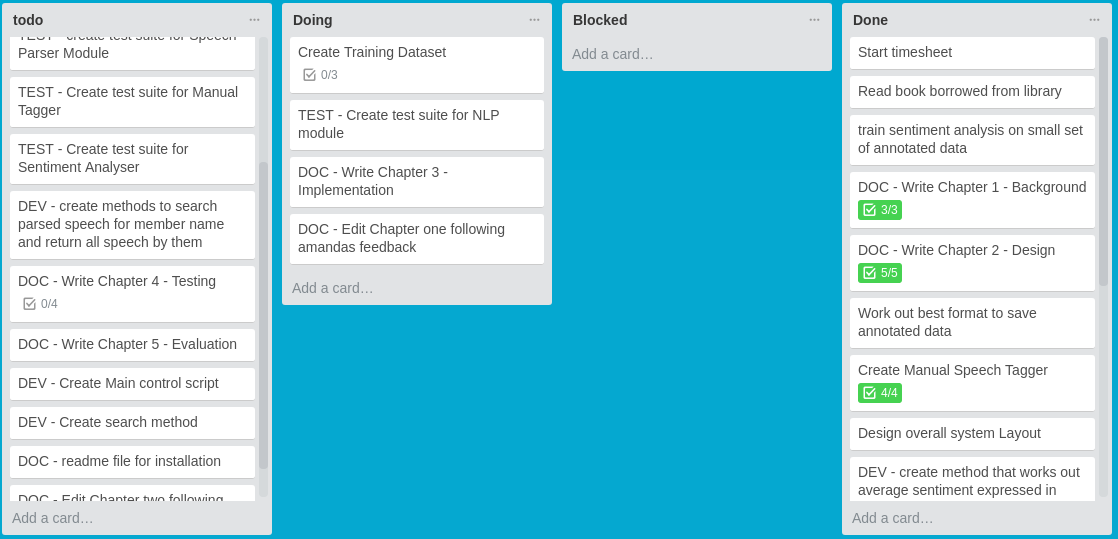
\includegraphics[width=\textwidth]{trello_board_screenshot}
	\caption{Screenshot of a Trello Board showing work in progress, done, and not yet started}
	\label{fig:trello_screenshot}
\end{figure}

In utilizing this tool for the organization of the project, development was planned out. Each "Card" of the board represented one task, and could be moved between columns. More complicated tasks were broken down into separate tasks, or a checklist could be added to a card, should the task need to remain as a single task for whatever reason.

\section{Conclusion}
Now that the background work has been documented, this report will move on to look at the design process of the project, documenting the choices made for each part of the project and the reasoning behind them, and showing some of the design work undertaken.